\section{The Conundrum of the Big Bang}

\begin{quotex}
This \emph{logos} holds always but humans always prove unable to ever understand it, both before hearing it and when they have first heard it. \emph{For though all things come to be in accordance with this logos}, humans are like the inexperienced when they experience such words and deeds as I set out, distinguishing each in accordance with its nature and saying how it is. But other people fail to notice what they do when awake, just as they forget what they do while asleep.
\flright{\textsc{Heraclitus}}
\end{quotex}


\paragraph{Cosmology}


In this video, \textit{The Universe: How did it get here \& why are we part of it?}\footnote{\url{https://www.youtube.com/watch?v=9wLtCqm72-Y}}, the Mathematical Physicist \textbf{Roger Penrose} and the Philosopher \textbf{William Lane Craig} discuss the origins of the Universe. Penrose starts from the assumption that only matter and energy exist, or said differently, particles and motion. That does not explain why matter and energy seem to follow well defined mathematical laws.

\begin{wrapfigure}{rt}{.3\textwidth}
	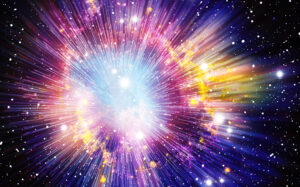
\includegraphics[width=.3\textwidth]{The-Big-Bang-Theory-of-Disruption-300x187.jpg}
\end{wrapfigure}

Like most mathematicians, Penrose is a Platonist. Specifically, he believes that mathematical truths are objectively and necessarily valid and are not merely mental constructions or social conventions. That is, mathematics belongs to Being. That explains why physical things must follow mathematical laws. The Kantian alternative is that maths is mind dependent only, so we can only make sense of the world insofar as it appears to follow mathematical laws. As a corollary to this view, phenomena that elude mathematical laws are incomprehensible. Summarizing, Penrose believes three things exist and the whole world can be explained by them: matter, energy, and the Platonic realm of mathematical ideas.

\paragraph{Life in the Big Bang}


That said, Penrose's description of the beginning of the Big Bang is intriguing. He points out that matter and energy are equivalent, according to the famous equation of the Theory of Relativity. At the beginning, matter has zero mass. Said another way, there is only energy in the form of photons. Then, Planck's equation relates the energy carried by a photon to its frequency. Therefore, at time 0, everything was vibration, which sounds like every New Age teaching. The photon energy\footnote{\url{https://en.wikipedia.org/wiki/Photon_energy}} was enormous, hence the electromagnetic frequency was also inordinately high, higher than anything we witness today.

Since we know that the entropy (the measure of disorder) of the universe is increasing, at time 0, there must have been no, or very little, entropy. After all, the entire creation of the universe had to be specified at the beginning, with all the laws of mathematics, physics, chemistry, biology, and so on, encoded. So how could that encoding come about?

Through the work initiated by \textbf{Claude Shannon} on information theory\footnote{\url{https://en.wikipedia.org/wiki/Information_theory}}, we understand that information is the opposite of entropy. The interesting fact is that the higher the frequency, the more information it can carry. That is why your cable Internet connection is faster than a modem connection, FM radio has better sound quality than AM radio, and 5g cellular service is faster that 4g; the former examples carry more information in the same unit of time.

Hence, at time zero, the frequency of the photons, acting as waves, was enormously high. It had to be, in order to hold all the information necessary to create our universe. For physics, this is a ``conundrum'', as described in \textit{Before the Big Bang: A Conundrum}\footnote{\url{https://accelconf.web.cern.ch/AccelConf/e06/PAPERS/THESPA01.PDF}}, although not particularly so for us. How exactly, did that information get there in the first place? The Ancients understood that the Logos was also in the beginning. just as was the Platonic realm of mathematics. For example, the Stoics regarded the \emph{logos spermatikos} as the generative principle of the Universe.


\paragraph{Conformal cyclic cosmology}


Penrose has developed a theory which he calls conformal cyclic cosmology (CCC). Since Penrose is all over youtube, information on CCC is readily available. I have no desire to refute his theory \emph{qua} physics, which may or not be true, but rather to draw out its metaphysical presupposition.

The CCC view is that the end of one universe is the beginning of another. So as a universe contracts, it creates the conditions for another one to arise. These universes are sequential, so the notion of ``before and after'' makes sense, despite the lack of a common time standard. This is unlike the multiverse theory that proposes that a new universe is created whenever there is a bifurcation in this universe. The CCC view seems tighter mathematically, as it does not require the spontaneous creation of a new universe. Moreover, in the CCC view, there is the possibility of information transfer from one universe to the next. One is tempted momentarily to suppose that the universes evolve by accumulating such information.

Guenon also claimed that metaphysically, the end of one universe is the beginning of the next. But he would reject any causal relationship between the two, since they do not have a common time reference, that is, there is no before and after.

The weakness of the CCC theory is that there is no first universe, so the chain goes back ad infinitum. In that case, our universe could not have happened yet, since there is an uncountable number of universes going back in the series. It is just Hilbert's Hotel\footnote{\url{https://www.youtube.com/watch?v=faQBrAQ87l4}} in reverse. I don't know how Penrose addressed that issue.\footnote{This has nothing to do with Kalam's argument.}

\paragraph{God and the Intelligibility of the Universe}


Since Penrose assumes that all the phenomena in the universe relates back to the Big Bang, Craig challenged him on the origin of life. Craig claims that the fundamental constants of physics, while not derived from any physical theory, are fine-tuned for the existence of life. Hence, there must be a God who makes that possible.

Penrose is not persuaded. First of all, he says, we really don't understand what life is, nor how different values for those constants would affect it. Truly puzzled, he just cannot see how such a God would alter his CCC theory; in other words, the mathematics remains the same.

Actually, neither can we. Craig is a neotheist, that is, he thinks that God is a being in time, rather than the traditional view that God is beyond being and time. Craig isn't very convincing because he treats God as a likely hypothesis rather than as necessary. That sounds like a scientific proposal to Penrose, so he asks how the God hypothesis can be falsified. I suppose by finding a universe in which the fundamental constants are such that intelligent could never have emerged. We sympathise with Schopenhauer when he asks where exactly is the Scientist in his theory. The physicist can only tell us what the universe might have ``looked like'' had he been there to observe it.

Although the CCC theory is a mathematical tour de force, it turns out that physics alone can account neither for the existence of life nor for consciousness. Forget about explaining the movement of atoms for a day in downtown Manhattan, not even in principle.

\url{https://www.youtube.com/watch?v=9wLtCqm72-Y} 

\flrightit{Posted on 2020-03-04 by Cologero}

\begin{center}* * *\end{center}

\begin{footnotesize}
\begin{sffamily}
\texttt{Geber on 2020-03-06 at 02:26 said:}

BB theory doesn't tell us anything about the cyclicity of the Universe and does not address a paradox: why the universe seems to return to the macrocoscopic state of minimum entropy that it had at the BB.

Sir Penrose claimed to have resolved this paradox by taking into account the information loss in BH which occurs in Hawking's black-hole evaporation and which allows an entropic renormalization. The Orch OR theory is associated with proto-conscious events and is panexperiential in nature which finds a parallel with the vedantine attributeless zero and undivided infinite consciousness. Both in CCC and in non-dualistic monism there is no ``external teleological agency'' that creates the universe while in qualified monism the macrocosm can be regarded as an organic unity of souls, matter and a centralised intelligence. Within the framework of absolute theism, the idea of God is conceptualised for anagogic purposes but is not regarded as a physical reality inasmuch as it does not have an ego or a separate existence. Both CCC and absolute monism assume an open position in regards to the hard problem of consciousness. Obviously, theories are based on empirical evidences which are only provisional for both, science and theology.

\hfill

\texttt{Cassiodorus on 2020-03-07 at 17:34 said:}

William Lane Craig certainly does not reject the doctrine of God's necessary being. So he is not a neotheist on that count. However, he could be called a neotheist insofar as he rejects Divine simplicity .

That said, it should be recognized that the distinction between ``neo'' and classical theism is not particularly important to the Perennialist perspective of Guenon. For the unqualified nondualist (like Guenon), theism of all stripes are at the level of saguna -- in the domain of relativity. Therefore even the God of classical theism is Maya or illusion.

\hfill

\texttt{Cologero on 2020-03-08 at 11:00 said:}

The question remains: where is Roger Penrose in all of this? Can \textit{Orchestrated objective reduction}\footnote{\url{https://en.wikipedia.org/wiki/Orchestrated_objective_reduction}} or
\textit{Conformal cyclic cosmology}\footnote{\url{https://en.wikipedia.org/wiki/Conformal_cyclic_cosmology}} predict Roger Penrose? Apparently, the universe wants to know itself through the physicist. And why do the microtubules that underlie consciousness care whether or not the theories are true?

\hfill

\texttt{CASSIO DORUS on 2020-03-08 at 13:42 said:}

William Lane Craig does not reject God as necessary being. However, he does reject Divine simplicity which could put him in the ``neotheist'' camp.

It should be noted that, from the Guenonian Perennialist perspective, the distinction between ``neo'' and classical theism is not particularly important and besides the point. The personal Creator of the theistic traditions is ``Saguna'' Brahman which is understood as the lower level of Divinity, that is, within the domain of relativity and ultimately, illusory.

\hfill

\texttt{CASSIO DORUS on 2020-03-09 at 13:01 said:}

How is the impossibility of an infinite regress a la Hilbert's Hotel not have anything to do with the Kalam? Isn't that precisely how the Kalam argument works?

\hfill

\texttt{Cologero on 2020-03-10 at 23:40 said:}

I don't believe I mentioned ``infinite regress''. Kalam's argument is metaphysical rather than mathematical.

It may work if the previous universes were smaller, but still conformal. Then the limit would to to 0 rather than to $-\infty$.

\hfill

\texttt{Cologero on 2020-04-03 at 13:04 said:}

Here is \textbf{St. Bonaventure} on infinite regress:

\textit{The Beginning of the World:} \url{https://www.gornahoor.net/?p=3957}


\hfill

\texttt{Max on 2020-09-06 at 08:10 said:}

An anecdote about the scientist in his theory.

There was once a refrigerator, about which I discovered that milk standing on the top shelf would go sour very quickly, while the rest of the items were fine. It took me a couple of months after first moving in to figure out that the lights must always be on, even with the door closed, which thus heated the uppermost compartment. After formulating my hypothesis, I unscrewed the lightbulb, and eagerly awaited the outcome of my experiment. Removing the lightbulb proved to eliminate the problem. There had been no way to identify the error by sensation alone, but only through exercise of reason and agency. Who knows how long the previous occupants must have endured living with the ``refrigerator-light error'', which turned out to be real and not only metaphorical in this case.

Would it have been possible to find the fault by help of physical measurements? Where would you even begin considering that there might be thousands of components? Perhaps by studying the technical drawings and measuring on the electrical circuits. The approach of troubleshooting by eliminating possible sources of error is much more effective however. Now we have only spoken about simple systems constructed by humans, but a comparison could be made to negative theology. Hoping to arrive at knowledge of God by examining every miniscule detail of physical nature seems unlikely.

In the discussion with Penrose, it was mentioned that the total mathematical possibilities are greater than what you would actually need in order to describe the laws of physics. If that which is non-physical is greater than that the physical, it means that knowledge is not reducible to physical structures. That can be verified by anyone of the requisite intellectual capacity.

\hfill

\texttt{Leonardo Cavalcanti on 2020-09-07 at 07:28 said:}

Brilliant. I wonder how come no one can understand this anymore, the level of thought today is so barren that even the highest authorities in ``science'' do not know where their ideas come from nor can they make sense of what they say. Yet most of these go unnoticed by the masses.

\end{sffamily}
\end{footnotesize}

